%; whizzy paragraph -pdf xpdf -latex ./whizzypdfptex.sh
%; whizzy-paragraph "^\\\\begin{frame}"
% latex beamer presentation.
% platex, latex-beamer でコンパイルすることを想定。 

%     Tokyo Debian Meeting resources
%     Copyright (C) 2009 Junichi Uekawa
%     Copyright (C) 2010 Nobuhiro Iwamatsu

%     This program is free software; you can redistribute it and/or modify
%     it under the terms of the GNU General Public License as published by
%     the Free Software Foundation; either version 2 of the License, or
%     (at your option) any later version.

%     This program is distributed in the hope that it will be useful,
%     but WITHOUT ANY WARRANTY; without even the implied warranty of
%     MERCHANTABILITY or FITNESS FOR A PARTICULAR PURPOSE.  See the
%     GNU General Public License for more details.

%     You should have received a copy of the GNU General Public License
%     along with this program; if not, write to the Free Software
%     Foundation, Inc., 51 Franklin St, Fifth Floor, Boston, MA  02110-1301 USA

\documentclass[cjk,dvipdfmx,12pt]{beamer}
\usetheme{Tokyo}
\usepackage{monthlypresentation}
%  preview (shell-command (concat "evince " (replace-regexp-in-string "tex$" "pdf"(buffer-file-name)) "&"))
%  presentation (shell-command (concat "xpdf -fullscreen " (replace-regexp-in-string "tex$" "pdf"(buffer-file-name)) "&"))
%  presentation (shell-command (concat "evince " (replace-regexp-in-string "tex$" "pdf"(buffer-file-name)) "&"))

%http://www.naney.org/diki/dk/hyperref.html
%日本語EUC系環境の時
\AtBeginDvi{\special{pdf:tounicode EUC-UCS2}}
%シフトJIS系環境の時
%\AtBeginDvi{\special{pdf:tounicode 90ms-RKSJ-UCS2}}

\title{東京エリア Debian 勉強会}
\subtitle{資料}
\author{岩松 信洋 iwamatsu@debian.org\\IRC nick: iwamatsu}
\date{2010年04月17日}
\logo{
\includegraphics[width=8cm]{image200607/openlogo-light.eps}}

\begin{document}

\frame{\titlepage{}}

\emtext{設営準備にご協力ください}

\begin{frame}
 \frametitle{勉強会の連絡事項}
\begin{minipage}[t]{0.45\hsize}
  \begin{itemize}
   \item 注意事項
	 \begin{itemize}
	  \item 飲食?
	 \end{itemize}
  \end{itemize}
\end{minipage} 
\begin{minipage}[t]{0.45\hsize}
 \begin{itemize}
  \item piuparts の使い方
  \item upstart 再入門
  \item debtags 入門
  \item Debian JP Project Leader からのありがたいお言葉
 \end{itemize}
\end{minipage}
\end{frame}


\begin{frame}
 \frametitle{前回のDebian勉強会}
\begin{minipage}[t]{0.45\hsize}
  \begin{itemize}
   \item 株式会社朝日ネット 
   \item 注意事項
         \begin{itemize}
          \item 飲食?
         \end{itemize}
  \end{itemize}
\end{minipage}
\begin{minipage}[t]{0.45\hsize}
 \begin{itemize}
  \item ニューラルネットワークで画像を分類してみた
  \item weka
  \item libfftw
  \item man-db 深追い
  \item dpkg v3 quilt
 \end{itemize}
\end{minipage}
\end{frame}

\begin{frame}{Hack Cafe}
 最近ハックカフェしてますか?\\
 毎週、新宿近辺で Debian Hack Cafe を行っているはずです。\\
 \url{http://twitter.com/debian_hackcafe}\\
\end{frame}

\emtext{事前課題}

\begin{frame}{事前課題}
\begin{enumerate}
 \item あなたの使っているinitは?
 \item あなたのパッケージ検索方法は?
\end{enumerate}
\end{frame}

{\footnotesize


\begin{prework}{ $B868}=(9/(B }

\begin{enumerate}
\item $B%G%U%)%k%H$N(B2$B$r;HMQ$7$F$$$^$9!#(B
$BDL>o$N%$%s%9%H!<%k$r$7$F$=$N$^$^;HMQ$7$F$$$k$+$i$G$9!#(B
2-5$BA4$FF1$8$J$N$KB>$N%i%s%l%Y%k$r;HMQ$9$k0UL#$O$o$+$C$F$$$^$;$s(B

\item apt-get apptitude$B!"!V%Q%C%1!<%8$NFbMF$r8!:w!W$r;HMQ$7$^$9!#(B
$BL@3N$KL>A0$,J,$+$k$b$N$O(Bapt-get$B$d(Bapptitude$B$G(B
$B$3$&$$$&$b$N$,$[$7$$$H;W$&$H$-$O!V%Q%C%1!<%8$NFbMF$r8!:w!W$r;H$$$^$9!#(B
$B%-!<%o!<%I$,;H$o$l$F$$$J$$%Q%C%1!<%8$G$b8!:w$9$k$3$H$,2DG=$@$+$i$G$9(B
\end{enumerate}

\end{prework}



\begin{prework}{ $B%-%?%O%i(B }
\begin{enumerate}

\item $B%G%U%)%k%H$GAH$_9~$^$l$k!V(Binit$B!W!"FC$KITET9g$,$J$$$?$a!#(B
\item $B:G6a$O!"!V(BGoogle$B@h@8!W$K?R$M$k;v$N$[$&$,B?$$!#(B

\end{enumerate}

\end{prework}



\begin{prework}{ yama1066 }
\begin{enumerate}

\item sysvinit
$B$^$@0\9T$7$F$J$$$+$i!#(B
upstart $B$K0\9T$9$k%a%j%C%H$,5DO@$G$-$l$P$$$$$J$H;W$$$^$9!#(B
\item dselect $B$G$R$?$9$i%4%j%4%j!D!"13$G$9!#(Bapt-cache search $B$G$[$2$[$2!#(B
\end{enumerate}

\end{prework}

\begin{prework}{ henrich }
\begin{enumerate}
\item sysvinit $B$r;H$C$F$^$9!#@N$O(B initng $B$r;H$C$?$3$H$b$"$j$^$7$?$,!D(B
$BLLE]$rHr$1$k$?$a!"$G$9$+$M!#(B
\end{enumerate}

\end{prework}



\begin{prework}{ koedoyoshida }

\begin{enumerate}
\item $B0BDj;V8~$J$N$G(Blenny$BI8=`$N(Binit$B$G$9!#(B
$B;E;v$G;H$C$F$k%^%7%s$O(Bupstart$B$d(Binit$B$,:.:_$7$F$$$^$9!#(B

$B;d$O4pK\E*$K(BLinux$B$O%5!<%P;HMQ$G$9!#(B
$BLGB?$K:F5/F0$7$J$$$N$G$"$^$j287C$r<u$1$F$$$^$;$s!#(B

$BFC$K%a!<%+!<7O$N%5!<%P5!$O(B($B:F(B)$B5/F0;~$K(BSAS,FC$BEy$r4^$a$?(BBIOS$B%A%'%C%/$@$1$G?tJ,$+$+$k$N$b$6$i$J$N$G!"5/F09bB.2=$N%a%j%C%H$O<u$1$K$/$$$H$$$&$N$,@5D>$J$H$3$m$G$9!#(B

init$B0J30$r;HMQ$9$k$3$H$K$h$k!"5/F0;~0J30$N%a%j%C%H$,M-$l$PCN$j$?$$$G$9!#(B

\end{enumerate}

\end{prework}



\begin{prework}{ $BNkLZ?rJ8(B }
\begin{enumerate}
\item sysvinit$B!#(B
$BFC$K%9%T!<%I$r5a$a$h$&$H;W$C$?$3$H$,$J$$$3$H$H!"%5!<%S%95/F0$,HsF14|$@$H2?$+LdBj$,5/$-$?$H$-$KD4::$7$K$/$$%$%a!<%8$,$"$k$?$a!#(B
$B$H$O$$$(!"(BUbuntu$B$N%^%7%s$G$O(BUpstart$B;H$C$F$$$k$N$G!"$?$@N.$5$l$F$$$k$@$1$@$H;W$$$^$9!#(B
\end{enumerate}

\end{prework}



\begin{prework}{ $BF#BtM}Ao(B(risou) }
\begin{enumerate}
\item $B:#;HMQ$7$F$$$k$N$O(B sysvinit $B$G$9!#M}M3$O!"(B lenny $B$N%G%U%)%k%H$K$J$C$F$$$k$+$i$G$9!D!D!#(B
$B!t$3$N$"$?$j!"0c$$$,$h$/$o$+$C$F$J$$$N$G!"$o$6$o$6JQ99$7$F$J$$$G$9!#(B
\end{enumerate}

\end{prework}



\begin{prework}{ $BB<ED?.?M(B }

\begin{enumerate}
\item sysvinit$B!#>/$7A0$K(BSqueeze$B$r%$%s%9%H!<%k$7$?$i%G%U%)%k%H$@$C$?$+$i!#(B
\item  apt-cache search$B$G$6$C$/$j$H8+Ev$r$D$1$F$+$i(Bapt-cache show$B$G>\:Y$r3NG'!#(B
\end{enumerate}
\end{prework}

\begin{prework}{ akedon }

\begin{enumerate}
\item sysvinit $B$G$9!#8=:_!"%G%U%)%k%H$J$N$H%a%+%K%:%`$,C1=c$J$N$G$3$l$GNI$$$+$J$H;W$C$F$$$^$9!#(B
\item aptitude search $B!A(B $B$H(B apt-file search $B!A(B $B$r;H$C$F$$$^$9!#(B
\end{enumerate}
\end{prework}

\begin{prework}{ Hirotaka Kawata }

\begin{enumerate}
\item init$B!#(BDebian $BI8=`$N(B init ($B$U$D$&$N(B init)
\item aptitude search "keyword"
\end{enumerate}
\end{prework}

\begin{prework}{ opentaka }

\begin{enumerate}
\item $B%G%U%)%k%H$N(Binit$B!#%G%U%)%k%H$GF~$C$F$$$?$N$G!#(B
\item aptitude search "package name"
\end{enumerate}
\end{prework}

\begin{prework}{ $B>>_7FsO:(B }
\begin{enumerate}
\item $B$"$^$j0U<1$7$F$$$^$;$s$G$7$?$,!"%G%U%)%k%H$N$b$N$r;H$C$F$$$^$9!#(Bsysvinit?
\item aptitude search hoge
\end{enumerate}
\end{prework}

\begin{prework}{ $B$^$($@$3$&$X$$(B }

\begin{enumerate}
\item sysvinit$B!#%F%9%H4D6-$H$+$G$O(Bupstart$B$b;n$7$F$^$9$,!"(BMacBook$B$N(BSid$B4D6-$H$+$G$O@Z$jBX$($k$N$^$@I]$$$G$9$M!#(B
\item apt-cache
\end{enumerate}
\end{prework}

\begin{prework}{ Yasunori Higashiyama }

\begin{enumerate}
\item sysvinit$B!#FC$K:$$C$F$$$J$$$N$G$=$N$^$^!#(B
\item web$B$G8!:w$+(Baptitude search
\end{enumerate}
\end{prework}

\begin{prework}{ $B4d>>(B $B?.MN(B }

\begin{enumerate}
\item sysvinit $B$G$9!#(BDebian$B$N%G%U%)%k%H$@$+$i$G$9!#(B
\item aptitude $B$G8!:w$7$F$$$^$9(B $B!#%?%0$r;H$$$^$9!#%Q%C%1!<%8$N%$%s%9%H!<(B
      $B%k$O(Bapt $B$G$9$,(B....$B!#$"$H$O!"(Biceweasel$B$d(BGoogle Chrome$B$N8!:w%\%C%/%9$G8!:w$9$k$3$H(B
      $B$b$"$j$^$9!#(B
\end{enumerate}
\end{prework}


\begin{prework}{ google-account@rolf.leggewie.biz }

$B:#2s$b$h$m$7$/$*4j$$$7$^$9!#(B

\end{prework}



}


\section{DWN quiz}
\begin{frame}{Debian 常識クイズ}

Debian の常識、もちろん知ってますよね?
知らないなんて恥ずかしくて、知らないとは言えないあんなことやこんなこと、
みんなで確認してみましょう。

今回の出題範囲は\url{debian-devel-announce@lists.debian.org} に投稿された
内容とDebian Project Newsからです。

\end{frame}

\subsection{問題}

\santaku
{DPL 2010 に立候補しているのは誰?}
{Yasuhiro Araki} % JP 
{Charles Plessy}
{Kurt Roeckx}
{B}

\santaku
{Debian policy 3.8.4.0で追加された項目は?}
{/sys と /selinux のFHSに対する例外ポリシー}
{kFreeBSDとLinuxを共存するポリシー}
{スーパ牛さんパワーに関するポリシー}
{A}

\santaku
{最近ハードウェアトラブルがあったサーバは?}
{rie.debian.org}
{ries.debian.org} % ftp-master.debian.org
{rise.debian.org }
{B}

\santaku
{buildd.debian.orgのあるサーバが移動しました。どこに移動したでしょう。}
{peri.debian.org} % ppc buildd
{cimarosa.debian.org} % 移動前
{grieg.debian.org} % 移動後
{C}

\santaku
{squeezeのインストーラで追加された機能は}
{Recommendsをインストールするようにします}
{インストーラ上でパッケージがビルドできます}
{クロスアーキテクチャインストール機能を追加しました}
{A}

\santaku
{新しくmips用porterboxが追加されました。CPUコア数はいくつでしょうか。}
{64}
{32}
{16}
{C}


% ------------------------------------------------------------------------------
\emtext{piuparts の使い方}
% ------------------------------------------------------------------------------

\begin{frame}{はじめに}
パッケージメンテナの簡易ワークフロー

\begin{figure}[h]
\includegraphics[height=0.6\hsize]{image201004/devwork.eps}
\label{fig:devwork}
\end{figure}

\end{frame}


\begin{frame}{忘れがちなテスト}
忘れがちなテスト
\begin{itemize}
\item アンインストールのチェック
\item クリーンインストールのチェック
\end{itemize}
\end{frame}

\begin{frame}{piuparts}
Piuparts\\
\begin{itemize}
\item インストールのチェック
\item アンインストールのチェック
\item アップグレードのチェック
\end{itemize}
\end{frame}


\begin{frame}[containsverbatim]{piupartsの使い方}

\begin{itemize}
\item ローカルPCにあるパッケージをチェックする\\
パッケージメンテナが使う
\item 既にDebianにインストールされているパッケージをチェックする\\
\texttt{piuparts.debian.org}で使う事が多い
\end{itemize}

\end{frame}

\begin{frame}[containsverbatim]{実行結果}
\begin{commandline}
$ sudo piuparts libcv4_2.0.0-4_i386.deb -l /tmp/libcv4_2.0.0-4_i386.piuparts-log
0m0.0s INFO: ------------------------------------------------------------------------------
0m0.0s INFO: To quickly glance what went wrong, scroll down to the bottom of this logfile.
0m0.0s INFO: FAQ available at http://wiki.debian.org/piuparts/FAQ
0m0.0s INFO: ------------------------------------------------------------------------------
0m0.0s INFO: piuparts version 0.38 starting up.
0m0.0s INFO: Command line arguments: /usr/sbin/piuparts libcv4_2.0.0-4_i386.deb -l /tmp/libcv4_2.0.0-4_i386.piuparts-log
0m0.0s INFO: Running on: Linux chimagu 2.6.31-1-686 #1
 SMP Sun Nov 15 20:39:33 UTC 2009 i686
0m0.0s DEBUG: Starting command: ['dpkg', '--info', 'libcv4_2.0.0-4_i386.deb']
0m0.2s DUMP:
.... 省略 .....
6m32.6s DEBUG: Starting command: ['chroot',
 '/tmp/tmplunhrZ', 'umount', '/proc']
6m32.6s DEBUG: Command ok: ['chroot',
 '/tmp/tmplunhrZ', 'umount', '/proc']
6m33.0s DEBUG: Removed directory tree at /tmp/tmplunhrZ
6m33.0s INFO: PASS: All tests.
6m33.0s INFO: piuparts run ends.
\end{commandline}
\end{frame}

\begin{frame}{piupartsの動作}
\begin{figure}[H]
%\begin{center}
\includegraphics[height=0.7\hsize]{image201004/piuparts-process.eps}
\label{fig:piuparts-process}
%\end{center}
\end{figure}

\end{frame}

\begin{frame}{ログの見方}

\begin{enumerate}
\item コマンド実行({\bf DEBUG: Starting command:})
\item 実行開始タグ({\bf DUMP:})
\item 実行時のログ
\item コマンド結果({\bf ERROR:} or {\bf DEBUG: Command ok})
\item テスト結果
\end{enumerate}
\end{frame}


\begin{frame}[containsverbatim]{テストが正常に終了した場合}

\begin{commandline}
.....省略.....
6m13.7s INFO: PASS: Installation and purging test.
.....省略.....
6m32.6s INFO: PASS: Installation, upgrade and purging tests.
.....省略.....
6m33.0s INFO: PASS: All tests.
6m33.0s INFO: piuparts run ends.
\end{commandline}
\end{frame}

\begin{frame}[containsverbatim]{エラーがある場合}

\begin{commandline}
0m6.0s DEBUG: Starting command: ['chroot', \
  '/org/piuparts.debian.org/tmp/tmpZ-SX9D',\
   'apt-get', '-y', 'install', 'upstart']
0m6.3s DUMP:
  Reading package lists...
  Building dependency tree...
  The following extra packages will be installed:
    libdbus-1-3
  Recommended packages:
    dbus
  The following packages will be REMOVED:
    sysvinit
  The following NEW packages will be installed:
    libdbus-1-3 upstart
  WARNING: The following essential packages will be removed.
  This should NOT be done unless you know exactly what you are doing!
    sysvinit
  0 upgraded, 2 newly installed, 1 to remove and 0 not upgraded.
  Need to get 636kB of archives.
  After this operation, 1196kB of additional disk space will be used.
  E: There are problems and -y was used without --force-yes
0m6.3s ERROR: Command failed (status=100): ['chroot', \
  '/org/piuparts.debian.org/tmp/tmpZ-SX9D', \
  'apt-get', '-y', 'install', 'upstart']
\end{commandline}
\end{frame}

\begin{frame}[containsverbatim]{piupartsのオプション}

\end{frame}

\begin{frame}[containsverbatim]{-p オプション}
pbuilderのbase.tgzをpiupartsで利用する

\begin{commandline}
$ sudo piuparts -p libcv4_2.0.0-4_i386.deb
\end{commandline}
\end{frame}

\begin{frame}[containsverbatim]{-d オプション}
テストするディストリビューションの指定
\begin{commandline}
$ sudo piuparts -d sid -d squeeze libcv4_2.0.0-4_i386.deb
.....
\end{commandline}
\end{frame}

\begin{frame}[containsverbatim]{- -apt オプション}
debianにインストールされているパッケージのテスト
\begin{commandline}
$ sudo piuparts --apt -d squeeze libcv4
\end{commandline}
\end{frame}

\begin{frame}[containsverbatim]{- -mirror オプション}
ミラーサーバの指定

\begin{commandline}
$ sudo piuparts -p libcv4_2.0.0-4_i386.deb --mirror http://debmirror.example.org/debian
\end{commandline}
\end{frame}

\begin{frame}[containsverbatim]{依存するパッケージの回避方法}
\begin{itemize}
\item パッケージの指定で回避する方法\\
依存するパッケージを一緒に指定する
\begin{commandline}
$ sudo piuparts -p libcv-dev_2.0.0-4_i386.deb libcv4_2.0.0-4_i386.deb
\end{commandline}

\item \texttt{*.changes}ファイルを指定する方法

\begin{commandline}
$ sudo piuparts -p opencv_2.0.0-4_i386.changes
\end{commandline}
\end{itemize}
\end{frame}

\begin{frame}[containsverbatim]{piuparts.debian.org}
\begin{itemize}
\item パッケージメンテナがインストール、アンインストール、アップグレード
      のチェックしない
\item パッケージ作成時はチェックしたが、環境の変化のよるエラーをトラッキ
      ングできていない
\item QA チームで\texttt{piuparts.debian.org}としてサービスを立ち上げた
\end{itemize}
\end{frame}


\begin{frame}[containsverbatim]{現在チェックエラーになっているパッケージ}

\begin{itemize}
\item タグ : piuparts
\item ユーザタグ : debian-qa@lists.debian.org
\end{itemize}
以下でチェック可能\\
\url{http://bugs.debian.org/cgi-bin/pkgreport.cgi?tag=piuparts;users=debian-qa@lists.debian.org}

\end{frame}

\begin{frame}[containsverbatim]{現在の問題点}

けっこう安定して動作している。

\begin{itemize}
\item チェック結果が適切ではない
\item マニュアル不備\\
\end{itemize}

\begin{commandline}
$ piuparts --help
.... 中略 ....
 -B FILE, --end-meta=FILE
                     XXX
\end{commandline}

\end{frame}

\begin{frame}[containsverbatim]{まとめ}
\begin{itemize}
\item ログは見にくいが、パターンを見ればわかる。
\item piuparts をテストパターンに組み込みこんで、テストしましょう。
\item v2 を開発中。開発はbzr上。\\
\url{http://code.liw.fi/piuparts2/bzr/trunk/}
\end{itemize}
\end{frame}


% ------------------------------------------------------------------------------
\emtext{upstart 再入門}
% ------------------------------------------------------------------------------

% ------------------------------------------------------------------------------
\emtext{debtags 入門}
% ------------------------------------------------------------------------------


% ------------------------------------------------------------------------------
\emtext{Debian JP Project Leader からのありがたいお言葉}
% ------------------------------------------------------------------------------

 
\begin{frame}{次回の勉強会}

\begin{itemize}
 \item 2010年5月21日: 筑波大学 \\
筑波大学 Linux User Group (つくらぐ) さんと合同開催です。

\end{itemize}
 
\end{frame}

\end{document}

;;; Local Variables: ***
;;; outline-regexp: "\\([ 	]*\\\\\\(documentstyle\\|documentclass\\|emtext\\|section\\|begin{frame}\\)\\*?[ 	]*[[{]\\|[]+\\)" ***
;;; End: ***
